% =========================================================
% CSC311 Final Project Report Template
% Single column, 12pt, 8 pages max.
% =========================================================

\documentclass[12pt]{article}

% ---------- Packages ----------
\usepackage[left=0.85in,right=0.85in,top=1in,bottom=0.85in]{geometry}
\usepackage{parskip}         % blank line between paragraphs, no indent
\setlength{\parskip}{6pt plus 1pt minus 1pt}
\usepackage{titlesec}
\titlespacing*{\section}{0pt}{14pt plus 2pt minus 2pt}{10pt plus 1pt minus 1pt}
\titlespacing*{\subsection}{0pt}{12pt plus 3pt minus 3pt}{8pt plus 2pt minus 2pt}
\usepackage{graphicx}
\usepackage{booktabs}
\usepackage{amsmath, amssymb}
\usepackage{siunitx}
\usepackage[hidelinks]{hyperref}
\usepackage{caption}
\usepackage{enumitem}
\usepackage{xcolor}
\usepackage{mathpazo}

%--------- Headers and footers ------
\usepackage{fancyhdr}
\pagestyle{fancy}
\setlength{\headheight}{14.49998pt}
\fancyhf{}
\fancyhead[L]{CSC311 Project Report}
\fancyhead[R]{Group 46915}
\fancyfoot[C]{\thepage}

% ---------- Captions & Lists ----------
\captionsetup{font=small, labelfont=bf}
\setlist[itemize]{noitemsep, topsep=2pt}
\setlist[enumerate]{noitemsep, topsep=2pt}

% ---------- Safe figure helper ----------
\makeatletter
\newcommand{\maybeincludegraphics}[3]{%
  \begin{figure}[h]
    \centering
    \IfFileExists{#1}{%
      \includegraphics[width=0.7\linewidth]{#1}%
    }{%
      \fbox{%
        \parbox[c][0.28\textheight][c]{0.7\linewidth}{%
          \centering
          \vspace{0.5em}
          \textit{[Placeholder for \texttt{#1}]}\\
          Add your figure here.
          \vspace{0.5em}
        }%
      }%
    }%
    \caption{#2}
    \label{#3}
  \end{figure}%
}
\makeatother

% =========================================================
% Title Page
% =========================================================
\begin{document}

\begin{titlepage}
    \centering
    \vspace*{3cm}

    {\Large {CSC311: Introduction to Machine Learning} \par}
    \vspace{1cm}
    
    {\Large {Project Report} \par}
    \vspace{1cm}
    
    {\large \textit{What's on the Canvas? Classifying Paintings from Survey Responses} \par}
    \vspace{3cm}
    
    {\large Submitted by \par}
    
    \vspace{0.5cm}
    {\large Group 46915}
    
    \vspace{0.5cm}
    {\large Qinyue (Alex) Li, Zhaotong (Macqueen) Pan, Qian (Angela) Su \par}
    
    \vfill
    {\large University of Toronto \\ Winter 2026 \par}
\end{titlepage}
\clearpage
\setcounter{page}{1}

% ================================================
% 2. Executive Summary
% ================================================
\section{Executive Summary}

We explored three model families for classifying survey responses into one of three paintings: K-Nearest Neighbors (KNN), Softmax Regression, and a Multi-Layer Perceptron (MLP). All models were trained on the same 14-feature set (numeric, Likert, multi-hot categorical, and TF-IDF text) and tuned via stratified GroupKFold 5-fold cross-validation with macro-F1 as the selection criterion. Our best-performing model is Softmax Regression (LBFGS, $C{=}1$), achieving a projected test accuracy of \textbf{89\%}. Softmax outperformed the MLP (88.2\%) and KNN (85.8\%) on the held-out test set, likely because the approximately linear class separation in our feature space favours a simpler model with fewer parameters to overfit, while KNN's distance-based approach struggles in the 172-dimensional feature space.

% ==================================================
% 3. Data Exploration
% ==================================================

\section{Data Exploration}
\subsection{Dataset Overview}
The target variable is Painting, which consists of three classes, each containing 562 observations (1686 total), resulting in a perfectly balanced class distribution. The dataset includes 14 input features of four types: 4 continuous numerical features (emotion intensity, number of objects noticed, number of prominent colours, willingness to pay), 4 ordinal categorical features measured on 5-point Likert scales (e.g., agreement with emotional statements), 3 nominal categorical features (preferred room, viewing companion, associated season), and 3 free-text response features (e.g., imagined soundtrack, painting description). Most numeric features are roughly unimodal with moderate spread, except willingness to pay, which is heavily right-skewed with values spanning from 0 to $10^{30}$ due to joke responses. Likert features show class-dependent response patterns (e.g., Figure~\ref{fig:sombre-bar}).

\subsection{Issues}
\begin{itemize}
\item Several features contain a small number of missing values, typically between 65 and 85 per feature (approximately 4–5 \% of the dataset).
\item Existence of outliers. For example, an extreme value (100) is observed in the feature ``How many prominent colours do you notice in this painting?''. For most features, we retain outliers: median imputation and z-score normalization already reduce their influence on model training, and removing them risks discarding legitimate responses. The willingness-to-pay feature is a special case: raw values span 30 orders of magnitude (from 0 to $10^{30}$) due to joke responses, causing the standard deviation to be ${\sim}2.6 \times 10^{28}$. After plain z-score normalization, all reasonable values collapse to approximately the same score, destroying the feature's discriminative power. We address this with a $\log(1+x)$ transform (see Pre-processing).
\item Inconsistencies. For features with mixed data types, some entries are numerical values while others include symbols or non-numeric text.
\end{itemize}

\subsection{Pre-processing}
\begin{itemize}
\item Missing value imputation. Numeric and Likert features are imputed using the median to reduce sensitivity to skewness and outliers. Missing nominal categorical entries are represented as all-zero multi-hot vectors (no category selected), which is the natural default for multi-select fields where the respondent may not have answered. (Our proposal planned most-frequent-response imputation for categorical features; we switched to all-zero vectors because multi-hot fields have no single ``most frequent'' category.)
\item Normalization. Numeric and Likert features are normalized to zero mean and unit variance to prevent large-range features from dominating distance calculations. Likert responses (e.g., ``4 - Agree'') are first parsed to their integer values (1--5) and then treated as numeric for imputation and normalization. 
\item Type consistency. The feature ``How much (in Canadian dollars) would you be willing to pay for this painting?'' is cleaned by removing currency symbols and non-numeric texts, then converting all entries to numerical values.
\item Outlier-robust pay transformation. After cleaning, negative pay values are clipped to 0, and the column is transformed via $\log(1+x)$ before z-score normalization. This compresses the 30-order-of-magnitude range into $[0, 69]$, producing a standard deviation of ${\sim}4.5$ and preserving the feature's ability to distinguish between classes. The $\log(1+x)$ function is parameter-free, so no training-set statistics are used in the transform itself; only the subsequent z-score statistics are fitted on training data.
\item Multi-hot encoding. Nominal categorical features (room, companion, season) allow multiple selections separated by commas. Each unique category becomes a binary indicator column, producing a multi-hot representation.
\item Text features. Missing text entries are treated as empty strings, yielding all-zero TF-IDF vectors. Text features are then transformed using TF-IDF, which converts text into numerical vectors while down-weighting common words.
\end{itemize}

\subsection{Data splitting}
All exploratory analysis, visualizations, and statistics reported in this section were computed exclusively on the training set to prevent information from the test set from influencing modelling decisions.

The dataset is divided into training and test sets, with 80\% of the data allocated to the training set and 20\% to the test set. Since each student contributes three related observations, group-based splitting (GroupShuffleSplit by student ID) is applied to ensure that all responses from the same student remain in the same partition, preventing cross-set data leakage. Hyperparameter selection is performed using stratified GroupKFold 5-fold cross-validation on the training set, where fold assignment also respects student groups so that no student's responses appear in both a training fold and a validation fold. All pre-processing transformations are fitted using only the training data (or training fold) and subsequently applied to the held-out set.

\subsection{Key insights about predictive features}
``How many objects caught your eye in the painting?'' is a continuous feature.
The boxplot (Figure~\ref{fig:objects-boxplot}) shows clear separation in medians and difference in spread across the three classes.
``This art piece makes me feel sombre'' is an ordinal categorical feature measured on a 5-point Likert scale (1 = Strongly disagree, 5 = Strongly agree). The stacked bar chart (Figure~\ref{fig:sombre-bar}) shows distinct response distributions across the three classes.

\begin{figure}[ht]
    \centering
    \begin{minipage}[t]{0.50\linewidth}
        \centering
        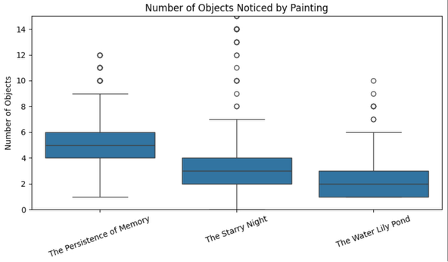
\includegraphics[width=\linewidth]{Figure1.png}
        \caption{Number of objects noticed in each painting}
        \label{fig:objects-boxplot}
    \end{minipage}\hfill
    \begin{minipage}[t]{0.45\linewidth}
        \centering
        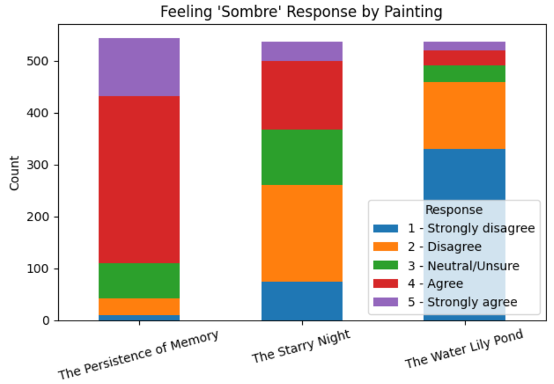
\includegraphics[width=\linewidth]{Figure2.png}
        \caption{Feeling sombre response for each painting}
        \label{fig:sombre-bar}
    \end{minipage}
\end{figure}

\subsection{Model choices}
The approximately monotonic class separation in key features (Figures~\ref{fig:objects-boxplot}--\ref{fig:sombre-bar}) suggests that a linear model such as \textbf{Softmax Regression} may already perform well. However, interactions across the four feature modalities (numeric, Likert, categorical, text) may create nonlinear boundaries, motivating an \textbf{MLP}. Finally, the clear clustering visible in Figure~\ref{fig:objects-boxplot} suggests that distance-based \textbf{KNN} can exploit local structure, while also serving as a non-parametric baseline to verify that the parametric models learn something beyond nearest-neighbour similarity.

% ====================================
% Methodology
% ====================================
\section{Methodology}

All three models share the same validation protocol: stratified GroupKFold 5-fold cross-validation on the training set, where fold assignment respects student groups to prevent within-CV data leakage. All preprocessing transformations are fitted on the training fold and applied to the validation fold.

\subsection{Softmax Regression}

\textbf{Reason:} Softmax regression~\cite{bishop2006prml} is a natural choice for multi-class classification when the features show approximately linear separation across classes, as observed in our data exploration. The model is simple, interpretable, and robust on small datasets. It uses all 14 input features (numeric, Likert, categorical, and TF-IDF text) to leverage the full feature set.

\textbf{Optimization Techniques:}
    \begin{itemize}
        \item \textbf{Optimizer}: LBFGS and SGD. We compare both to determine which optimizer works better on our feature set.
        \item \textbf{Regularization}: L2 regularization
        \item \textbf{Early Stopping Strategies:} For LBFGS, early stopping is not required since the softmax objective is convex and LBFGS converges to a global minimum. For SGD, we set \texttt{max\_iter}$=$1000.

    \end{itemize}
\textbf{Hyperparameters and Rationale:}
    \begin{itemize}
        \item LBFGS: L2 regularization strength $C = 1/\lambda \in \{0.1, 1, 10\}$ and convergence tolerance \texttt{tol} $\in \{10^{-3}, 10^{-4}, 10^{-5}\}$. Max iterations fixed at 2000 as a safeguard.
        \item SGD: L2 regularization $\alpha \in \{0.001, 0.0001, 0.00001\}$, learning rate schedule $\in$ \{optimal, constant, adaptive\}, initial learning rate $\eta_0 \in \{0.1, 0.01, 0.001\}$.
    \end{itemize}
\textbf{Hyperparameter tuning process:} Grid search over 9 LBFGS and 21 SGD configurations, evaluated using macro-F1 on each validation fold. The best optimizer and its hyperparameters are selected jointly.

\textbf{Deviation from proposal:} Our proposal planned SGD with step or exponential decay schedules. We implemented Softmax Regression using \texttt{sklearn.LogisticRegression} (LBFGS) and \texttt{SGDClassifier}, which provide \texttt{optimal}, \texttt{constant}, and \texttt{adaptive} learning rate schedules instead. These serve the same purpose of controlling step size during training and are the natural choices within the sklearn framework.

\subsection{Multi-Layer Perceptrons(MLP)}

\textbf{Reason:}
Multi-layer perceptrons~\cite{bishop2006prml,hastie2009esl} are suitable for this task because the dataset contains both
continuous features (emotion intensity, number of objects, number of colors) and high-dimensional categorical/text features (room preference, feelings, soundtrack descriptions, etc., after one-hot encoding or TF-IDF),
which together form a nonlinear feature space.

\textbf{Optimization Techniques:}
    \begin{itemize}
        \item \textbf{Optimizer:} Adam (via \texttt{sklearn.MLPClassifier})
        \item \textbf{Regularization:} L2 regularization (weight decay parameter $\alpha$)
        \item \textbf{Early Stopping:} Monitored validation loss; stopped training when no improvement was observed for 5 consecutive epochs (patience$=$5), with \texttt{max\_iter}$=$200 as an upper bound.
    \end{itemize}

\textbf{Deviations from proposal:} Our proposal planned to test dropout $\in \{0.0, 0.1, 0.2\}$, custom learning rate schedules (cosine and step decay), and number of epochs $\in \{20, 30, 40, 60\}$. We implemented the MLP using \texttt{sklearn.MLPClassifier}, which does not support dropout or custom LR schedules. Instead, we rely on L2 regularization and early stopping for overfitting control, and Adam's built-in adaptive learning rate. This is a reasonable substitute: L2 regularization penalizes large weights similarly to dropout's noise injection, and Adam already adapts per-parameter step sizes, reducing the need for an explicit schedule. Removing dropout, LR schedule, and epoch count from the grid also reduced the search space from the proposal's ${\sim}1400$ configurations to 120, addressing TA feedback that the original grid was impractically large for 5-fold CV.

\textbf{Hyperparameters and Rationale:}
    \begin{itemize}
        \item Hidden layer architectures $\in \{(32), (64), (128), (64{,}32), (128{,}64)\}$: single-layer and two-layer configurations with ${\sim}1350$ training samples. Deeper networks would likely overfit.
        \item Learning rate $\in \{0.01, 0.001\}$: Adam's adaptive step sizes work well in this range.
        \item L2 regularization $\lambda \in \{0.0001, 0.001, 0.01\}$: spans light to moderate weight decay to control overfitting without underfitting.
        \item Activation function $\in \{\text{ReLU}, \text{tanh}\}$: ReLU is the default for efficient gradient flow; tanh can work better on normalized inputs.
        \item Batch size $\in \{32, 64\}$: smaller batches add noise that can help regularization; both are reasonable for this dataset size.
    \end{itemize}
\textbf{Hyperparameter tuning process:} Grid search over all 120 combinations, evaluated using macro-F1 on each validation fold.

\subsection{K-Nearest Neighbors (KNN)}

\textbf{Reason:} KNN is a non-parametric baseline that classifies by majority vote among the $k$ nearest training points~\cite{hastie2009esl}, making no assumptions about decision boundary shape. Our 172-dimensional feature space (${\sim}1350$ samples) risks the curse of dimensionality~\cite{bishop2006prml}, but we include KNN to test whether the clear per-class clustering observed in data exploration overcomes this limitation.

\textbf{Optimization Techniques:}
    \begin{itemize}
        \item \textbf{Optimizer:} Not applicable. KNN has no trainable parameters and therefore requires no optimization procedure. 
        \item \textbf{Regularization:} The value of $k$ controls the bias--variance tradeoff: a small $k$ gives more flexible (but noisier) predictions, while a large $k$ smooths things out at the cost of potentially missing local structure. We search over a range of $k$ values to find the right balance.
    \end{itemize}
\textbf{Hyperparameters and Rationale:}
    \begin{itemize}
        \item Number of neighbours $k \in \{3, 5, 7, 11, 15, 21\}$: odd values avoid ties in majority voting. The range covers the typical bias--variance tradeoff from highly local ($k{=}3$, 0.2\% of training samples) to smoothed ($k{=}21$, 1.6\%).
        \item Distance metric $\in$ \{Euclidean, Manhattan\}: Euclidean penalizes large deviations more heavily; Manhattan is more robust to occasional outliers.
        \item Weighting scheme $\in$ \{uniform, distance\}: distance weighting lets closer neighbours have more influence, which can help when the class boundary falls within the neighbourhood.
    \end{itemize}
\textbf{Hyperparameter tuning process:} Grid search over all 24 combinations, evaluated using macro-F1 on each validation fold.

\subsection{Evaluation Metrics}
We use three complementary metrics to evaluate and compare all models:
\begin{itemize}
    \item \textbf{Accuracy} measures the overall proportion of correct predictions. Because our dataset is perfectly balanced (562 samples per class), accuracy is a meaningful metric that is not distorted by class imbalance.
    \item \textbf{Macro-F1 score} averages the F1 score across all three classes, where each class's F1 is the harmonic mean of its precision and recall. This is useful because accuracy alone can look fine even if the model does poorly on one particular painting; macro-F1 would drop in that case, making the problem visible. We use macro-F1 as the primary criterion when selecting hyperparameters during cross-validation.
    \item \textbf{Per-class precision and recall} are reported alongside macro-F1 to diagnose which classes, if any, are systematically misclassified.
\end{itemize}

\subsection{Implementation}
All three models were trained and tuned using scikit-learn
(\texttt{KNeighbors\-Classifier}, \texttt{Logistic\-Regression},
\texttt{SGD\-Classifier}, \texttt{MLP\-Classifier}).
Text features were vectorized with \texttt{Tfidf\-Vectorizer}.
For the final prediction script (\texttt{pred.py}), we exported the trained
Softmax weights, intercept, preprocessing statistics, and TF-IDF
vocabularies, then reimplemented the full pipeline and softmax inference using
only \texttt{numpy} and \texttt{pandas}, as required by the submission constraints.

% ===========================================
% 5. Results
% ===========================================
\section{Results}\label{sec:results}

Table~\ref{tab:comparison} compares the best configuration from each model family after grid search. KNN ($k{=}5$, Euclidean, distance weighting) achieves a CV macro-F1 of 0.808; its performance drops for $k \geq 11$, consistent with the bias--variance tradeoff. For Softmax, LBFGS ($C{=}1$, tol$=10^{-3}$) and the best SGD configuration ($\alpha{=}0.001$, adaptive, $\eta_0{=}0.1$) achieved nearly identical test macro-F1 (0.890 vs.\ 0.891); we selected LBFGS for its deterministic convergence. The best MLP (128-64, ReLU, lr$=$0.01, $\alpha{=}0.001$, batch size 64) achieved the highest CV macro-F1 of 0.890, but Softmax achieved the best test macro-F1 (0.890), suggesting the MLP's additional capacity slightly overfits on this dataset size.

\begin{table}[h]
\centering
\small
\caption{Comparison of best models across all three families.}\label{tab:comparison}
\begin{tabular}{@{}lcccc@{}}
\toprule
Model & CV Macro-F1 & Train Acc & Test Acc & Test Macro-F1 \\
\midrule
KNN ($k{=}5$, Euclidean, distance)       & 0.808 & 97.5\% & 85.8\% & 0.858 \\
Softmax (LBFGS, $C{=}1$, tol$=10^{-3}$) & 0.873 & 92.2\% & 89.1\% & 0.890 \\
MLP (128-64, ReLU, $\alpha{=}0.001$)     & 0.890 & 95.3\% & 88.2\% & 0.880 \\
\bottomrule
\end{tabular}
\end{table}

\textbf{Overfitting analysis.} The train--test accuracy gaps in Table~\ref{tab:comparison} reveal different degrees of overfitting across models. KNN shows the largest gap (97.5\% $\to$ 85.8\%, $\Delta{=}11.7\%$), consistent with the curse of dimensionality~\cite{bishop2006prml}: in 172 dimensions, the neighbourhood around each point is sparse and training neighbours are unreliable proxies for test-time neighbours. The MLP's gap ($\Delta{=}7.1\%$) is moderate, indicating that its extra capacity memorizes some training patterns that do not generalize. Softmax has the smallest gap ($\Delta{=}3.1\%$), confirming that the linear model generalizes best on this dataset.

\textbf{Error analysis.} Across all three models, \textit{The Starry Night} is the hardest class: its test F1 is 0.79 (KNN), 0.84 (Softmax), and 0.83 (MLP). The Softmax confusion matrix (Figure~\ref{fig:softmax-cm}) shows that Starry Night errors are nearly evenly split between Persistence of Memory (9~samples) and Water Lily Pond (10~samples), suggesting that Starry Night shares feature characteristics with both other classes. The overlap with Persistence of Memory likely stems from shared strong emotional responses (e.g., high sombre agreement, as shown in Figure~\ref{fig:sombre-bar}). The Softmax model's per-class test metrics are: Persistence 0.92/0.89/0.91, Starry Night 0.85/0.83/0.84, Water Lily Pond 0.90/0.95/0.92 (precision/recall/F1).

\begin{figure}[h]
    \centering
    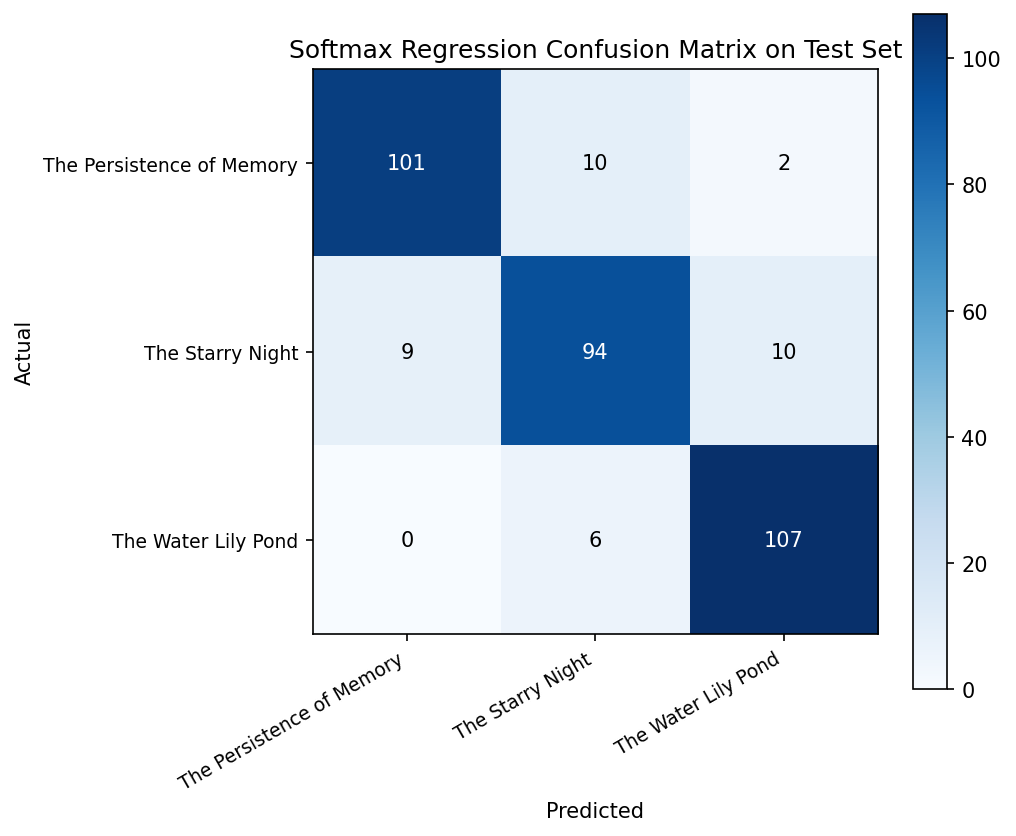
\includegraphics[width=0.45\linewidth]{softmax_confusion_matrix.png}
    \caption{Softmax Regression confusion matrix on the held-out test set.}
    \label{fig:softmax-cm}
\end{figure}

\textbf{Final model and test performance estimate.} We select Softmax Regression as our final model for the prediction script. We estimate its accuracy on the unseen test set to be \textbf{89\%}. The CV macro-F1 (0.873) and held-out test macro-F1 (0.890) are close, indicating stable generalization with no sign of overfitting. Despite the MLP achieving a higher CV macro-F1 (0.890), its test macro-F1 (0.880) falls below Softmax's, consistent with the principle that simpler models can generalize better when the training set is small (${\sim}1350$ samples) relative to the feature space (172 dimensions).

% ================================================
% 8. Contributions and Learning
% ================================================
\section{Contributions and Learning}

\begin{itemize}
    \item \textbf{Angela Su:} Implemented the KNN model (methodology, tuning, and evaluation), the evaluation metrics framework, and \texttt{pred.py}; wrote most of the final report. The most important lesson I learned is that the bias--variance tradeoff directly manifests in KNN through the choice of $k$: small $k$ overfits to noisy neighbours while large $k$ loses the local structure that makes KNN effective.
    \item \textbf{Macqueen Pan:} Implemented the softmax regression model, including hyperparameter tuning and final evaluation on the test set. Developed the preprocessing pipeline. The most important lesson I learned is that preprocessing must be consistent between the training set and unseen data to avoid data leakage and ensure fair evaluation.
    \item \textbf{Alex Li:} Implemented the MLP regression model, including hyperparameter tuning and final evaluation on the test set. Developed the basic methodology for MLP and Softmax. The most important lesson I learned is that sklearn MLPClassifier does not have drop rate choice input.
\end{itemize}

% ==================================================
% 9. References
% ==================================================
\bibliographystyle{plain}
\bibliography{references}

\end{document}
